\section{Overview}
\label{sec:overview}

As stated in \cref{ssec:goals}, one of the design goals during the project was
to keep the implementation of the REPL IDE-agnostic. To achieve this goal, the
product has been split into a backend and several frontends. The backend
interacts with the Spoofax services on behalf of the frontends. An overview of
its design can be found in \cref{fig:uml-overview}. A diagram of the complete
design can be found in \cref{cha:uml-diagram}.

\begin{figure}[h!]
  \centering
  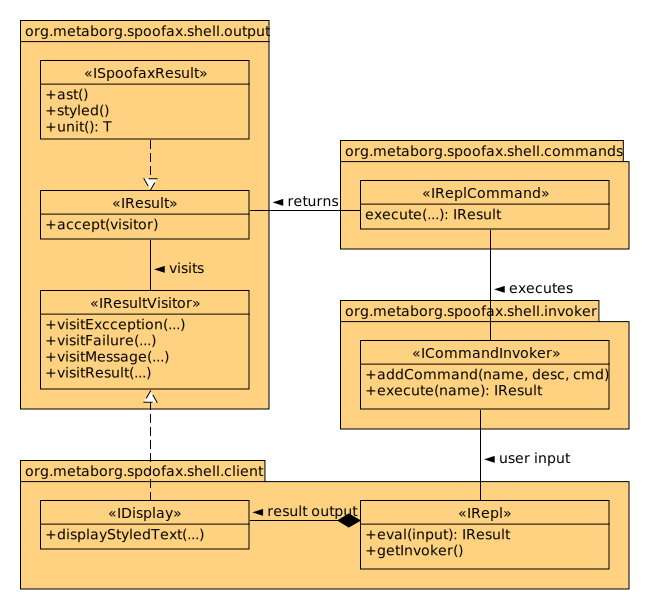
\includegraphics[width=0.75\textwidth]{uml-overview}
  \caption{An overview of the most relevant components of the backend.}
  \label{fig:uml-overview}
\end{figure}

To request and receive results from the backend, a frontend can invoke commands
by sending the command name and its parameters to the \texttt{ICommandInvoker}
in the backend. The \texttt{ICommandInvoker} will then execute the
\texttt{IReplCommand} corresponding to the command name. Every executed command
returns an \texttt{IResult}.

To execute a command, the frontend thus only has to implement a way of querying
the user for input, after which it can send this input to the
\texttt{ICommandInvoker}. Since execution of different commands can have
varying types of results, the actual returned type of \texttt{IResult} can
vary. The returned \texttt{IResult} can be visited by the frontend, thereby
dispatching results based on their specific types.


